\chapter{Cantidad de movimiento lineal}

\vspace{1.50cm}

\noindent Si imaginas la situación  en la que se hace chocar un auto contra una pared, y además también se hace colisionar una pelota de béisbol a la misma pared con la misma velocidad, entonces nos parece muy intuitivo decir que el auto causará mas daño a la pared a comparación de la pelota, dado que intuitivamente se sabe que el auto posee mucho mayor masa que la pelota. Pero uno preguntarse ¿Existe alguna manera de hacer que la pelota logre hacer el mismo daño que hizo el auto?, pués y si hacemos que esa pelota tenga una velocidad muy alta de tal modo que se logre ese mismo daño.\\

\noindent Pues parece que tanto la masa y la velocidad de un cuerpo son importantes para analizar situaciones en las que existen colisiones. Entonces ¿cómo codificamos la acción combinada de estas dos cantidades?, la respuesta es sencilla es la siguiente\\

\begin{tcolorbox}
Se define a la cantidad de movimiento $\vec{p}$ de un cuerpo como la simple multiplicación de su masa $m$ (cantidad escalar) por su velocidad $\vec{v}$ (cantidad vectorial):
\begin{center}
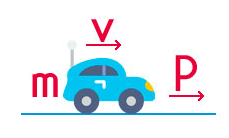
\includegraphics[scale=0.5]{images/figura1.png} 
\end{center}

\centering
\begin{center}
\begin{equation*}
\large{
\text{Cantidad de movimiento: }\quad \vec{p} = m\vec{v}
}
\end{equation*}
\end{center}

\large{¡¡  Esta cantidad es muy importante para la Física !!}
\end{tcolorbox} 
\vspace{0.5cm}

Podemos notar que la cantidad de movimiento al ser la multiplicación de una cantidad escalar (la masa) por una vectorial (la velocidad) resulta ser una cantidad vectorial. Por otro lado, en cuantos las unidades en las que la medimos\\ 

\vspace{0.2cm}
\begin{tcolorbox}
(unidades de medida de $\vec{p}$) = (unidades de medida de $m$) $\times$ (unidades de medida de $\vec{v}$)\\

es decir\\

\begin{center}
(unidades de medida de $\vec{p}$) = $kg\frac{m}{s}$.
\end{center}
\end{tcolorbox}
\vspace{0.2cm} 
 
\textbf{¿Por qué es tan importante esta cantidad?}\\

Resulta que esta cantidad se conserva en todo sistema cerrado, es decir, esta cantidad no cambia en un sistema que no interactúa  con el exterior. Y es así, que en realidad a esta conservación se la conoce como \textbf{Principio de la conservación de la cantidad de movimiento}, que junton con el principio de la conservación de la energía son reglas que se cumplen en todo proceso físico, como por ejemplo  en una colisión.\\

Para la resolución de problemas como lo son las colisiones podemos plantear este principio de la siguiente manera:

\vspace{0.2cm}
\begin{tcolorbox}
\textbf{Principio de conservación de la cantidad de movimiento:}

En un sistema en ausencia de fuerzas externas (sistema cerrado) la cantidad de movimiento se conserva.
 
\begin{center}
$\vec{p_{\text{inicio}}} = \vec{p_{\text{final}}}$. 
\end{center}

\end{tcolorbox}
\vspace{0.2cm}

Veamos unos pequeños ejemplos en donde podríamos aplicar este nuevo conocimiento

\vspace{0.2cm}
\begin{tcolorbox}
Volviendo al caso del auto que choca contra una pared, si suponemos que la masa de ese auto es de 3.4 toneladas y choca contra la pared a una velocidad de $72 km/h$, de modo que tendra una cantidad de movimiento

\begin{equation*}
p_{auto}= m_{auto}\times v_{auto}= 3400 kg \times 20\frac{m}{s}= 68000 kg\frac{m}{s}
\end{equation*}  

, así nos resulta cuestionarnos, ¿Qué velocidad debe imprimirse a una pelota de béisbol de 142 gramos de tal manera que tenga la misma cantidad de movimiento de auto?\\

\begin{equation*}
\text{Como sabemos que } p_{auto}=p_{pelota}=m_{pelota}\times v_{pelota},\text{entonces:}
\end{equation*}

\begin{equation*}
v_{pelota}=\frac{p_{auto}}{m_{pelota}}=\frac{68000 kg\frac{m}{s}}{0,142 kg}= 1,72\times 10^{6} \frac{km}{h}  
\end{equation*}
\end{tcolorbox}
\vspace{0.2cm}

Abordemos otro ejemplo 

\vspace{0.2cm}
\begin{tcolorbox}
Supongamos que lanzamos la misma pelota a la pared pero con una velocidad de 80 km/h, y de alguna manera vemos que esa pelota rebota en dirección cortraria a como la lanzamos con una velocidad de 45 km/h. ¿Cuál es entonces la cantidad de movimiento que absorvio la pared?\\

Para ello calculemos primero cual fue la cantidad de movimiento inicial de la pelota

\begin{equation*}
\vec{p_{inicio}} = m_{pelota}\times v_{inicio}= 0,142 kg\times 80 \frac{km}{h} = 11.36 kg \frac{km}{h}\quad \vec{i}
\end{equation*}

y la cantidad de movimiento de la misma pelota al final

\begin{equation*}
\vec{p_{\text{final}}} = m_{pelota}\times v_{\text{final}}= -0,142 kg\times 45 \frac{km}{h} = -6,39 kg \frac{km}{h} \quad \vec{i}
\end{equation*}

notese que esta cantidad de movimiento es negativa ya que la pelota rebota en dirección opuesta al inicio, de modo que la cantidad de movimiento que absorbe la pared es exactamente la cantidad de movimiento que pierde la pelota

\begin{equation*}
\vec{p_{\text{abssorbida}}}= \vec{p_{\text{final}}}-\vec{p_{\text{inicio}}}=--6,39 kg \frac{km}{h} \quad \vec{i}-11.36 kg \frac{km}{h} \vec{i}= -17.75 kg \frac{km}{h}\quad \vec{i}
\end{equation*}

\end{tcolorbox}

\newpage
Otro ejemplo clásico es

\vspace{0.2cm}
\begin{tcolorbox}

Supongamos que se dispara una bala de cañon con una velocidad de $120 km/h$, y si sabemos que esa bala de cañon pesa 5 kg y el cañon en sí 200 kg, ¿podemos encontrar la velocidad con que retrocede el cañon al disparar la bala?\\

La respuesta es sí, de hecho el principio de conservación de la cantidad de movimiento nos ayudará a encontrarla. Primero, notemos que antes de disparar la bala, el sistema estás en resposo, de modo que su cantidad de movimiento es 

\begin{equation}
\vec{p_{\text{total inicio}}} = m_{sistema}\times v_{inicio}= \vec{0} 
\end{equation}

y ya que la cantidad de movimiento de movimiento del sistema al inicio tiene que ser la misma despúes que se dispara la bala dado que tiene que cumplirse el principio de conservación de la cantidad de movimiento. Entonces veamos que cantidad de movimiento tiene la bala:

\begin{equation}
\vec{p_{bala}} = m_{bala}\times \vec{v_{bala}}= 5 kg\times 120 \frac{km}{h} \vec{i}= 600 kg\frac{km}{h}\quad \vec{i}
\end{equation}

ahora la del cañon:

\begin{equation*}
\vec{p_{\text{cañon}}} = m_{\text{cañon}}\times \vec{v_{\text{cañon}}}= 200kg\times \vec{v_{\text{cañon}}} 
\end{equation*}

entonces la cantidad de movimiento total del sistema al disparar la bala es

\begin{equation*}
p_{\text{total final}}= \vec{p_{bala}} + \vec{p_{\text{cañon}}} = 600 kg\frac{km}{h}\quad \vec{i}+ 200kg\times \vec{v_{\text{cañon}}}
\end{equation*}

entonces ahora si apliquemos el principio de conservación de energía

\begin{equation*}
p_{\text{total inicio}} = p_{\text{total final}}
\end{equation*}

de lo cual

\begin{equation*}
\vec{0} = 600 kg\frac{km}{h} \vec{i}+ 200kg\times \vec{v_{\text{cañon}}}
\end{equation*}

así

\begin{equation}
\vec{v_{\text{cañon}}}= -\frac{600 kg\frac{km}{h}\quad \vec{i}}{200 kg}= -3 \frac{km}{h}\quad \vec{i}
\end{equation}

de lo que se puede ver la velocidad del cañon tiene signo negativo, lo cual nos indica que el cañon se movió en sentido contrario al que salió la bala.

\end{tcolorbox}
\vspace{0.2cm}

Entonces te proponemos resolver el siguiente problema en clase o en casa.

\vspace{0.5cm}
\begin{tcolorbox}
Una partícula de masa 0.3 kg moviéndose a 0.5 m/s choca contra otra partícula de masa 0.4 kg que está en reposo. Después del choque la primera partícula se mueve a 0.3 m/s en una dirección que hace un  ángulo de 40o con la dirección original. Hallar la velocidad de la segunda partícula.
\end{tcolorbox}
